\documentclass[sigconf]{acmart}

\usepackage{hyperref}

%\usepackage{endfloat}
%\renewcommand{\efloatseparator}{\mbox{}} % no new page between figures

\usepackage{booktabs} % For formal tables

\settopmatter{printacmref=false} % Removes citation information below abstract
\renewcommand\footnotetextcopyrightpermission[1]{} % removes footnote with conference information in first column
\pagestyle{plain} % removes running headers


\begin{document}
\title{Big Data Analytics for Social Media Threat Intelligence}


\author{Tousif Ahmed}
\orcid{HID237}
\affiliation{%
\institution{Indiana University}
  \streetaddress{150 S Woodlawn Avenue}
  \city{Bloomington} 
  \state{Indiana} 
  \postcode{47405}
}
\email{touahmed@indiana.edu}



\begin{abstract}
Social media has become a virtual society for everyone where billions of people are interacting every day. With the humongous number of users, it has become extremely difficult to manage and track the user's behavior in social media.  Malicious actors leverage this weakness of social media platforms and target regular users with threats that include cyberbullying, malware distribution, spam distribution, fake news, and propaganda.  The consequence of such threats can affect a large number of people and can result in catastrophic damage. However, identifying the malicious users from the huge number of regular users remain the most challenging problem for the social media platforms. Big data analytics can be one of the most powerful tools for the social media platforms to prevent such attacks on social media platforms. This paper discusses the threats of social media and the ways to use big data analytics to prevent such attacks on social media platforms. 

\end{abstract}

\keywords{E534, HID 237,  Big Data, Social Media, Threat Intelligence, Privacy}


\maketitle





\section{Introduction}
More than two billion people use various social media platforms every day~\cite{social-media}. In every minute, approximately one million people logs into Facebook, 50,000 photos are uploaded on Instagram, half million tweets are posted on Twitter, two million snaps are created, and one million profile matches happen on Tinder (Figure ~\ref{f:socialmedia}) ~\cite{social-media2}. Social media platforms have become a virtual society for everyone where people are interacting with a large number of an audience every day. Similar to the regular society, there are bad actors in the virtual society who are trying to harm people. Due to the extended outreach, social media platforms have become an ideal platform for the malicious actors to harm that includes cyberbullying ~\cite{Slonje:2013,Kwan:2013,Singh:2017,Cheng:2017,HosseinmardiMRH15} and the distribution of offensive, misleading, false or malicious information ~\cite{Menczer:2016, socialbots-CACM, Shao15hoaxy, Shao17hoaxybots}. Terrorist and government can also leverage social media to spread propaganda~\cite{Aro2016, Weimann:2006}.


\begin{figure}[!ht]
 \centering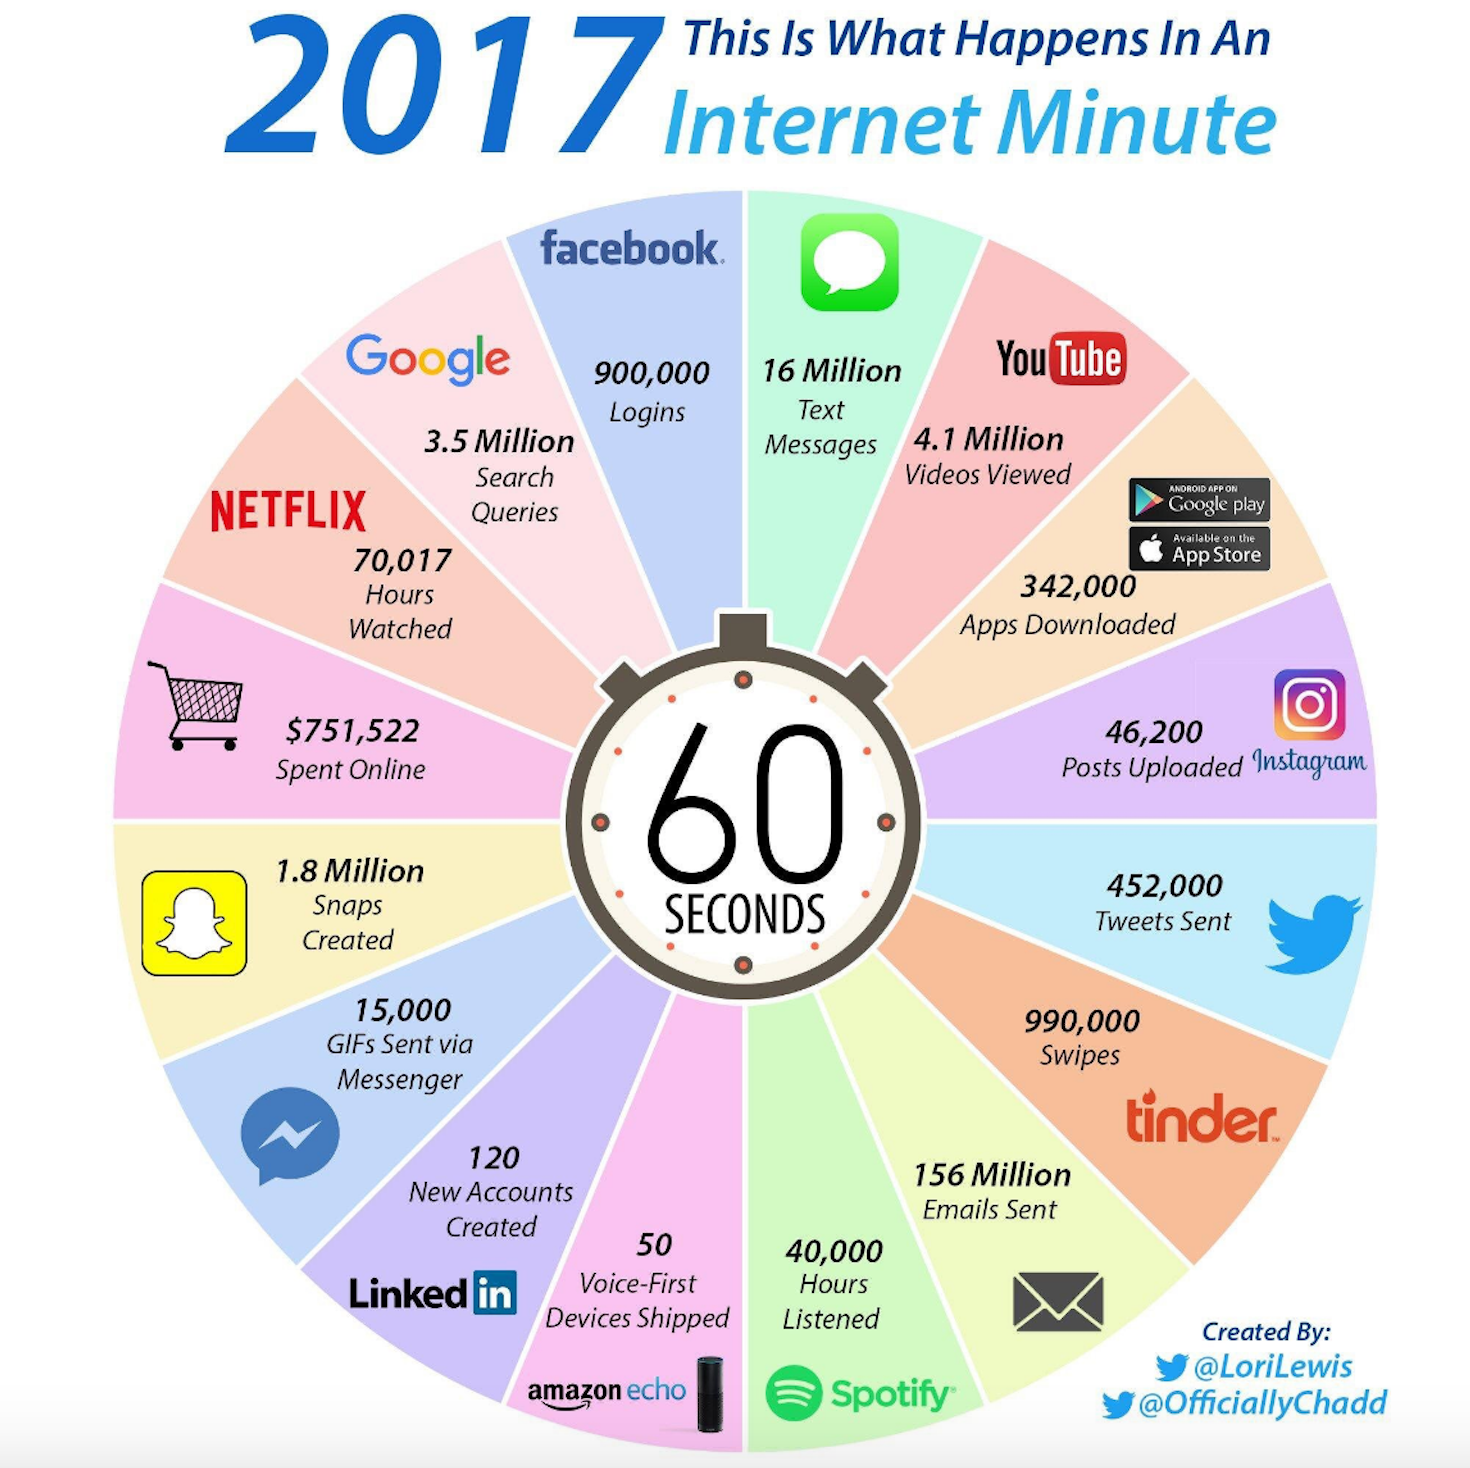
\includegraphics[width=0.5\columnwidth]{images/one-internet-minute.png}
  \caption{What happens in an internet minute?~\cite{social-media2}}\label{f:socialmedia}
\end{figure}

Since the beginning of society, malicious actors are common phenomena and society has taken necessary steps to control them. Law enforcement organizations have been helping the society to control social menaces and protect the individuals from internal and external threats.  Real society constituted by small groups, therefore, it is easier to control them. In contrast to the actual society, it is far more difficult to manage the virtual society due to its volume. It is nearly impossible to construct virtual law enforcement organizations in the virtual world and protect the individuals from malicious actors. Therefore, protecting the social media platforms from threats remain one of the most challenging problems. The recent advancement of machine learning and big data shows promises and offer a new set of weapons to fight. Big data analytics provides an easier way to scale, manage, and visualize user's data which can be valuable for fighting malicious actors. The volume of data gives the researchers tremendous insight which can be a new way to help regular users. 

There are a plethora of risks that Social Medias are facing every day. However, some threats can impact the user's safety and security. For that reason, generally, these platforms invest significant resources to prevent that. As already discussed earlier, regular analytics might not be fruitful to prevent such thing at scale, big data analytics gives more power to the providers and shows significant promises. This paper discusses four such safety and security threats and discusses how big data analytics have been used to reduce the impact. 

\section{Social Media Threat Intelligence}
This section discusses the impact of big data on social media threat intelligence. Each threat were discussed first then the use of big data on detecting and preventing the threats was discussed:

\subsection{Cyberbullying detection and identification}
Cyberbullying can be defined as the use of computing devices to hurt or embarrass another person.  Cyberbullying in social media constitutes posting negative or offensive comments in posts, post videos or photos to make fun of others,  stalking, harassing, and trolling.  Approximately, 43 percent teenagers in the U.S have been victims of cyberbullying in 2013 and most of them were bullied in social media~\cite{cyberbullying}. Cyberbullying has a bad impact on people, which include deep emotional trauma, mental disorder, substance abuse, and suicidal tendency~\cite{cb-effect}. 

The rise of social media has caused significant growth in cyberbullying. The rise of photos and social media have aggravated the situation. However, text analysis or social media post analysis has become impressively smart to detect cyberbullying~\cite{HosseinmardiMRH15}. Natural language processing algorithms like LDA can easily detect social media posts with negative meanings and keyword matching can be helpful to detect and identify the offensive keywords. Recent results show promising advancement in detecting cyberbullying and in future it would be far easier to control. Another potential approach to detect and identify cyberbullying is analyzing photos or videos.

\subsection{Information Abuse detection}
Although social media abuse falls in the category of cyberbullying, abuse can be different than cyberbullying. Social media abuse can be defined as misusing user's personal information that does not necessarily harm the user but can break the level of mutual trusts between the abuser and the abused. For example, stealing one's content from their social media profile does not harm the user but breaks the mutual trust in the relationship. In social media, people connect with others by putting a level of trust on others. Sometimes, bad actors can use the information to impersonate the person on social media. Later, the impersonated account can be used to embarrass or demean the victim. This might not be necessary causing mental harm to the victim but misusing the trust. Such bad actors are pretty common in social media. Since the bad actor's are using genuine information, it is very difficult to detect them.

One approach to detecting the abusers is to monitor the user's activity. Most of the cases, such actors exhibit some common behavior such as sending friend requests to random people, infrequent usage, random or anomalous behavior and such other behaviors. However, it is not possible for people to monitor the activity of the users to detect the abusers. However, common patterns can be helpful to detect such anomalies and data mining algorithms like k-means can be used to detect such anomalies. Big data analytics can also be helpful to blacklist the social media abusers and additional manual research can be useful to detect the abusers and ban them. For example, Xiao et al. ~\cite{Xiao:2015:DCF:2808769.2808779} utilized Apache Hive to build a fake profile detection system and using Hadoop streaming they monitored the newly registered dataset. Blacklisted users then sent for manual reviewing. Likewise, other social media platforms adopted similar approach to detect the abusers. 

\begin{figure}[!ht]
 \centering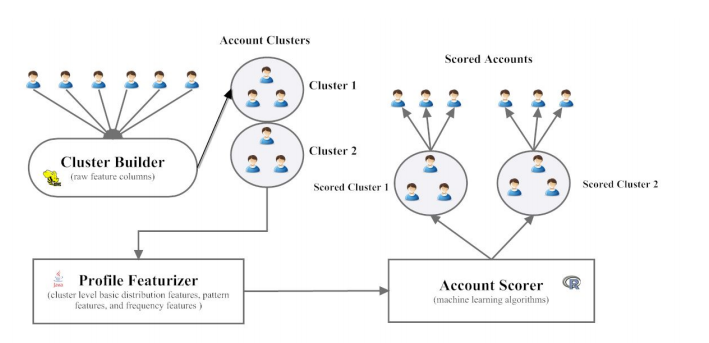
\includegraphics[width=\columnwidth]{images/fakeuser.png}
  \caption{Fake User detection approach used by LinkedIn\cite{Xiao:2015:DCF:2808769.2808779}}
  \label{f:fake}
\end{figure}


\subsection{Identifying the fake news/misinformation }
Various terrorist and government organization utilizes social media to spread their propaganda. Often, these organizations use fake news or false information to spread their agenda or to deceive people~\cite{Aymanns:2017}.  Since fake news is often hard to identify people often deceived by them and share the news. Due to its large volume of users, fake news can spread significantly fast and can impact the society. According to a survey conducted by pew research center, approximately one-fourth of the U.S. adults have shared fake news~\cite{fake2}. Analysts and evidence suggested that Russian government set up numerous fake accounts to spread dubious information regarding U.S. election 2016 and eventually impacted the U.S. election~\cite{fake2, Allcott:2017}.  Due to the significant impact on an organization, identifying fake news detection and prevention garnered significant attention from the researchers.

By leveraging new machine learning tools, now it has become easier to track the online spread of misinformation and detecting social bots~\cite{Shao17hoaxybots, Shao15hoaxy}. Fact checking using knowledge graph can check facts in nearly run-time which can be useful to identifying fake news quickly and prevent misinformation ~\cite{Shiralkar2017Finding-Streams}. More works use machine learning approaches to detect and prevent misinformation.



\subsection{Preventing Terrorism}
Various terrorist organizations like Al-Qaeda and ISIS use social media platforms to communicate with their members. They often use social media platforms to recruit new members~\cite{terrorism}. Due to the volume, now the impact of terrorism can be catastrophic and the increasing number of terrorist attacks on U.S and European countries proves that terrorists are becoming successful. Terrorism existed before and it exists now. But, modern technology has become a powerful tool for the terrorist organizations to amplify the impact. 

Counterterrorism organizations need massive surveillance to prevent the terrorists from harming people. Without the help of Big Data, it will be impossible to support such massive surveillance. Moreover, a proper design of surveillance tools can be useful to maintain the privacy of regular citizens. Big data analytics has significant contribution to make this happen. Data visualization tools can help the counterterrorism organizations to monitor such surveillance.



\section{Conclusion}
This paper briefly discusses the cybersecurity and safety risks on various social media and explored some existing Big data approaches to tackle such problem. New tools have already been successful to prevent and control various threats on social media, but it needs more research and additional tools. In near future, the threats can increase significantly and big data analytics need to be prepared for that to prevent future threats.



\begin{acks}

The authors would like to thank Professor Gregor von Laszewski for helping us with the instruction and resources that were required to complete this paper. We would also to like to thank the associate instructors for being available on the course website all the time and helping us with their answers.

\end{acks}



\bibliographystyle{ACM-Reference-Format}
\bibliography{report} 

\end{document}
